\documentclass{IEEEtran}
\usepackage{cite}
\usepackage{amsmath,amssymb,amsfonts}
\usepackage{algorithmic}
\usepackage{graphicx}
\usepackage{textcomp}
\def\BibTeX{{\rm B\kern-.05em{\sc i\kern-.025em b}\kern-.08em
    T\kern-.1667em\lower.7ex\hbox{E}\kern-.125emX}}
\begin{document}

\title{Compact quadrifilar helix antenna with embedded feed network}
\author{Dmitriy A. Dyomin, Ivan V. Filatov, Nikolay P. Chubinsky}
\maketitle
\begin{abstract}
  A compact quadrifilar helical antenna with embedded feeding circuit
  is presented in this paper.
\end{abstract}

\section{Introduction}
\label{sec:introduction}
Compact circularly polarized antennas with broad radiation pattern are widely used in many
communication systems including telecommand transmission channels for small satellite
applications. For example, circular polarized antennas are used for GNSS and GLONASS
operation. There is a wide variety of antennas that have circular polarization, the most commony
used are

\begin{itemize}
\item patch antennas
\item helical (including quadrifilar helix) antennas
\item turnstile antennas
\end{itemize}

Polarization of a simple helical antenna strongly depends on its geometry. Thin antennas
(circumference $C < 0.5 \lambda$) is excited by a normal mode and radiates lineary polarized
wave. However, generation of CP wave requires larger diameter ($C \approx \lambda$). This demand may
be relaxed if in case of quadrifilar helix antennas (QHA). They have an exceptional property of
radiating CP wave regardless of it's diameter.

Each class of these antennas may be further subdivided into two major subclasses:
\begin{itemize}
\item self-phased antennas
\item with external phasing circuits
\end{itemize}

Self-phasing is a techinque that allows generation of circular polarized (CP) wave using two
orthogonal linear polarized sources. These sources are tuned to resonate at above and below the
central frequency so that phase shift between the sources is $90^{\circ}$ at central
frequency. Provided the currents in these sources are equal, such system generates CP wave if fed by
single source without need in any external splitters and phasing circuits. This method is widely
used in building CP antennas of all the mentioned types. It has the advantage of simplicity and low
cost. However, self-phased antennas are usually narrowband (less that 1 percent) not just in terms
of return loss: their axial ratio (AR) degrades rapidly with offset from center frequency.

Another option is a phasing circuit. There are several demands to the feed network:
\begin{itemize}
\item equally split input power between output ports
\item provide phase progression of $90^{\circ}$ between adjacent ports
\item provide impedance matching between source and loads.
\end{itemize}

\begin{figure}
  \centering
  \centerline{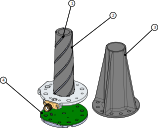
\includegraphics[width=0.95\linewidth]{images/QHA_Exploded}}
  \caption{QHA exploded view. Four helix arms (1) reside inside grooves on inner dielectric cone
    (2). This assembly is in turn covered by outer dielectric cone (3) and is placed on the aluminum
    case. Helices and SMA connector are soldered to the ports of the PCB (4).}
  \label{fig:exploded_view}
\end{figure}

\begin{figure}
  \centerline{\includegraphics{images/Sparam}}
  \caption{Simulated and measures return loss of the feed network with
    attached QHA. Center frequency for both plots is $F_c = 2.08~GHz$,
    calculated bandwidth is $BW_{calc} = \pm 3.6 \%$, measured
    bandwidth is $BW_{meas} = \pm 3.8 \%$}
  \label{fig:sparam}
\end{figure}

\begin{figure*}
  \centerline{\includegraphics{images/Directivity}}
  \caption{Directivity}
  \label{fig:directivity}
\end{figure*}
\end{document}
%%% Local Variables:
%%% mode: latex
%%% TeX-master: t
%%% End:
